\documentclass[twoside]{article}

%
% This is a borrowed LaTeX template file for lecture notes for CS267,
% Applications of Parallel Computing, UCBerkeley EECS Department.
% Now being used for CMU's 10725 Fall 2012 Optimization course
% taught by Geoff Gordon and Ryan Tibshirani.  When preparing 
% LaTeX notes for this class, please use this template.
%
% To familiarize yourself with this template, the body contains
% some examples of its use.  Look them over.  Then you can
% run LaTeX on this file.  After you have LaTeXed this file then
% you can look over the result either by printing it out with
% dvips or using xdvi. "pdflatex template.tex" should also work.
%

\setlength{\oddsidemargin}{0.25 in}
\setlength{\evensidemargin}{-0.25 in}
\setlength{\topmargin}{-0.6 in}
\setlength{\textwidth}{6.5 in}
\setlength{\textheight}{8.5 in}
\setlength{\headsep}{0.75 in}
\setlength{\parindent}{0 in}
\setlength{\parskip}{0.1 in}

%
% ADD PACKAGES here:
%

\usepackage{amsmath,amsfonts,graphicx}

%
% The following commands set up the lecnum (lecture number)
% counter and make various numbering schemes work relative
% to the lecture number.
%
\newcounter{lecnum}
\renewcommand{\thepage}{\thelecnum-\arabic{page}}
\renewcommand{\thesection}{\thelecnum.\arabic{section}}
\renewcommand{\theequation}{\thelecnum.\arabic{equation}}
\renewcommand{\thefigure}{\thelecnum.\arabic{figure}}
\renewcommand{\thetable}{\thelecnum.\arabic{table}}

%
% The following macro is used to generate the header.
%
\newcommand{\lecture}[4]{
   \pagestyle{myheadings}
   \thispagestyle{plain}
   \newpage
   \setcounter{lecnum}{#1}
   \setcounter{page}{1}
   \noindent
   \begin{center}
   \framebox{
      \vbox{\vspace{2mm}
    \hbox to 6.28in { {\bf Econ 626: Quantitative Methods II
  \hfill Fall 2018} }
       \vspace{4mm}
       \hbox to 6.28in { {\Large \hfill Lecture #1: #2  \hfill} }
       \vspace{2mm}
       \hbox to 6.28in { {\it Lecturer: #3 \hfill Scribes: #4} }
      \vspace{2mm}}
   }
   \end{center}
   \markboth{Lecture #1: #2}{Lecture #1: #2}

   %{\bf Note}: {\it LaTeX template courtesy of UC Berkeley EECS dept.}

   {\bf Disclaimer}: {\it Zhikun is fully responsible for the errors and typos appeared in the notes.}
   \vspace*{4mm}
}
%
% Convention for citations is authors' initials followed by the year.
% For example, to cite a paper by Leighton and Maggs you would type
% \cite{LM89}, and to cite a paper by Strassen you would type \cite{S69}.
% (To avoid bibliography problems, for now we redefine the \cite command.)
% Also commands that create a suitable format for the reference list.
\renewcommand{\cite}[1]{[#1]}
\def\beginrefs{\begin{list}%
        {[\arabic{equation}]}{\usecounter{equation}
         \setlength{\leftmargin}{2.0truecm}\setlength{\labelsep}{0.4truecm}%
         \setlength{\labelwidth}{1.6truecm}}}
\def\endrefs{\end{list}}
\def\bibentry#1{\item[\hbox{[#1]}]}

%Use this command for a figure; it puts a figure in wherever you want it.
%usage: \fig{NUMBER}{SPACE-IN-INCHES}{CAPTION}
\newcommand{\fig}[3]{
      \vspace{#2}
      \begin{center}
      Figure \thelecnum.#1:~#3
      \end{center}
  }
% Use these for theorems, lemmas, proofs, etc.
\newtheorem{theorem}{Theorem}[lecnum]
\newtheorem{lemma}[theorem]{Lemma}
\newtheorem{proposition}[theorem]{Proposition}
\newtheorem{claim}[theorem]{Claim}
\newtheorem{corollary}[theorem]{Corollary}
\newtheorem{definition}[theorem]{Definition}
%\newtheorem{example}[theorem]{Example}
\newenvironment{proof}{{\bf Proof:}}{\hfill\rule{2mm}{2mm}}
\newenvironment{example}{{\bf Example:}}{\hfill\rule{2mm}{2mm}}

\newtheorem{remark}[theorem]{Remark}
%\newenvironment{remark}[1][Remark]{\begin{trivlist}\item[\hskip \labelsep {\bfseries #1}]}{\end{trivlist}}


% **** IF YOU WANT TO DEFINE ADDITIONAL MACROS FOR YOURSELF, PUT THEM HERE:

\newcommand\E{\mathbb{E}}
\newcommand\dd{\mathrm{d}}

\usepackage{hyperref}
\usepackage{cancel}
\usepackage{listings}
\usepackage{amssymb}
\newcommand\pp{\partial}
\newcommand\pd{\partial}
\newcommand\imp{$\Longrightarrow$}
\newcommand\lb{\left (}
\newcommand\rb{\right )}
\newcommand\lsb{\left [}
\newcommand\rsb{\right ]}
\newcommand\lcb{\left \{}
\newcommand\rcb{\right \}}
\newcommand\R{\mathbb{R}}

\begin{document}
%FILL IN THE RIGHT INFO.
%\lecture{**LECTURE-NUMBER**}{**DATE**}{**LECTURER**}{**SCRIBE**}
\lecture{8}{Continue on Dynamic Programming}{Prof. Daniel Levy}{Zhikun Lu}
%\footnotetext{These notes are partially based on those of Nigel Mansell.}
\footnotetext[1]{Visit \url{http://www.luzk.net/misc} for updates.}

\hfill Date: September 7, 2018

\underline{Metrics on a set of functions}

Let $X$ be a set of continuous functions that map $[a,b] \to \mathbb{R}$. Then, $\forall f, g \in X$, we can define
\begin{enumerate}
    \item Sup-metric
    \begin{equation}
        d_{sup}(f,g) \equiv \sup_{x \in [a,b]} |f(x)-g(x)|
    \end{equation}
    \item $L^{2}$-metric
    \begin{equation}
        d_{2}(f,g) \equiv \left(\int_{a}^{b} \left[ f(x) - g(x) \right]^{2}  \dd x  \right )^{\frac{1}{2}}  
    \end{equation}
\end{enumerate}

\begin{lemma}
    Let $C$ be a set of continuous real-valued functions defined on $[a,b] \subset \mathbb{R}$. Prove that $(C,d)$ is a metric space if $d(f,g) = \sup_{x \in [a,b]} |f(x)-g(x)|$.
\end{lemma}
\begin{proof}
    \begin{enumerate}
        \item $d(f,g) = \sup |...| \geq 0$ by properties of absolute value.
        \item $d(f,g) = \sup_{x \in [a,b]} |f(x)-g(x)| \iff f(x) = g(x), \forall x \in [a,b].$
        \item $d(f,g) = \sup_{x \in [a,b]} |f(x)-g(x)| = \sup_{x \in [a,b]} g(x)-f(x)| = d(g,f)$ 
        \item $$\begin{aligned}
            d(f,h) 
            &= \sup_{x \in [a,b]} |f(x)-h(x)|\\
            &= \sup_{x \in [a,b]} |f(x)-g(x)+g(x)-h(x)|\\
            &\leq \sup_{x \in [a,b]} \Big \{ |f(x)-g(x)| + |g(x)-h(x)| \Big \}\\
            &\leq \sup_{x \in [a,b]} |f(x)-g(x)| + \sup_{x \in [a,b]} |g(x)-h(x)|\\
            &= d(f,g) + d(g,h)
        \end{aligned}$$
    \end{enumerate}
\end{proof}
 
 \begin{theorem}[Banach space theorem, a version of SLP pp.47-49]
    Let $B(X) \subseteq F(X)$ be the set of bounded functionals that map from $X$ to $\R$. Then:
    \begin{enumerate}
        \item $||f|| = \sup_{x\in X} |f(x)|$ is a norm on $B(X)$.
        \item $B(X)$ is a normed linear space.
        \item $B(X)$ is a Banach space.
    \end{enumerate}
 \end{theorem}
\begin{proof}
    \begin{enumerate}
        \item From the def of $||f|| = \sup_{x\in X} |f(x)|$ it follows that
        \begin{itemize}
            \item [a)] $||f|| \geq 0$ be properties of absolute value.
            \item [b)] $||f|| = 0$ if $f$ is the zero functional: $f(x) = 0 ~ \forall x$
            \item [c)] $||\alpha f || = |\alpha| ||f||$
            because
            \[
            || \alpha f|| = \sup |\alpha f(x)| = \sup \{ |\alpha| |f(x)| \} = |a| \sup |f(x)|
            \]
            \item [d)] $||f+g|| = \sup\limits_{x\in X} |(f+ g)(x)| = \sup |f(x) + g(x)| \leq \sup \{ |f(x)| + |g(x)|\} \leq \sup \{ |f(x)|\} + \sup \{|g(x)|\}  = ||f|| + ||g|| $
        \end{itemize}
        \item $\forall f \in B(X)$ and $\forall \alpha \in \R$,
            \[
            \alpha f(x) \leq |\alpha| ||f(x)|| ~\forall x \in X \Longrightarrow \alpha f(x) \in B(X) ~ \forall \alpha \in \R
            \]
            $\forall f,g \in B(X)$, $(f+g)(x) = f(x) + g(x) \leq ||f(x)|| + ||g(x)||$ \imp $B(X)$ is closed under addition and scalar multipliation, i.e., $B(X)$ is a subspace of $F(X)$, i.e., $B(X)$ is a normed linear space.
        \item To show that $B(X)$ is a Banach space, we need to show that $B(X)$ is complete. 

        Assume that $\{f_{n}\}$ is a Cauchy sequence in $B(X)$.

        \underline{Note}: Another way of defining a Cauchy sequence is as follows: A sequence in a metric space $(X,d)$ is Cauchy if $\forall n,m \in \mathbb{N}$, $\lim\limits_{\substack{
            n \to \infty\\
            m \to \infty}
            } d(x_{n},x_{m}) = 0$.

        Then, $\forall x \in X$,
        \[
        |f_n(x) - f_{m}(x)| \leq ||f_n - f_m|| \longrightarrow 0
        \]
        because the RHS is the supremum, and because $f_{n}(x)$ is Cauchy sequence. 

        Therefore, $\forall x \in X$, $f_n(x)$ is a Cauchy sequence of real numbers. Since $\R$ is complete, this sequence converges: $f(x) \equiv \lim_{n \to \infty} f_{n}(x)$. 

        To show that $||f_n - f|| \to 0$:

        Since $f_{n}$ is Cauchy, let $\epsilon > 0$ and $N \in \mathbb{N}$ s.t.
        \[
        ||f_{n}- f_{m} || < \frac{\epsilon}{2}, ~ \forall m,n > N
        \]
        Then $\forall x \in X$ and $ \forall n > N$, 
        \[
        |f_n(x) - f(x)| \leq |f_n(x) - f_m(x)| + |f_m(x) - f(x)| \leq ||f_n - f_m|| + ||f_m - f||
        \]
        By choosing $m$ (which might depend on $x$) suitably, each term on RHS can be made smaller than $\frac{\epsilon}{2}$ and therefore $|f_n(x)-f(x)| < \epsilon ~ \forall x \in X$ and $\forall n > N$. Since this ($< \epsilon$) is true for all $x \in X~\forall n > N$, it will be true for the sup as well.

        \imp $||f_n- f|| = \sup |f_n(x) - f(x)| < \epsilon$.

        \imp $f = \lim_{n\to \infty} f_n$. Obivously, $||f||$ is finite.

        \imp $f \in B(X).$
    \end{enumerate}
\end{proof}

\section{Contraction Mappting}
Let $(S, \rho)$ be a metric space and $T:S \to S$ be operator. $T$ is a \underline{contraction mapping} with modulus $\beta$ if for some $\beta \in (0,1)$, $\rho(T(x),T(y) \leq \beta \rho(x,y), ~ \forall x,y \in S$.

\underline{Contraction coefficient} is the infimum of all these $\beta$'s.

\begin{example}
    $S = [a,b] \subset \R$, $\rho(x,y) = |x- y|$
\end{example}

\begin{theorem}
    $T: [a,b] \to [a,b]$ is a contraction if for some $\beta \in (0,1)$,
    \[
    \frac{T(x)-T(y)}{|x-y|} \leq \beta < 1, \quad \forall  x, y \in [a,b], ~x\neq y
    \]
\end{theorem}

\begin{example}
    $T(x) = \frac{x}{2}$
    \[
        \rho(T(x), T(y)) = \rho\left (\frac{x}{2}, \frac{y}{2} \right ) = \left |\frac{x}{2} - \frac{y}{2} \right | = \frac{1}{2} \left | x-y \right | = \frac{1}{2} \rho(x,y)
    \]
    \imp $T$ is a contraction mapping with $\beta = \frac{1}{2}$.
    \begin{center}
    \texttt{[Insert a graph here]}
    \end{center}
\end{example}

\begin{theorem}[Uniform Continuity of Contraction Mappting]
    If $T:S \to S$ is a contraction in a metric space $(S,d)$, then it is uniformly continuous.
\end{theorem}
\begin{proof}
    $T:S\to S$ is uniformly continuous if $\forall \epsilon > 0$, $\exists \delta(\epsilon) > 0$, s.t. $\forall x,y \in S, ~ d(x,y) < \delta \Longrightarrow d(T(x),T(y)) < \epsilon$.

    Since $T$ is contraction, we know that $\exists \beta \in (0,1)$ s.t. $d(Tx,Ty) \leq \beta d(x,y), ~ \forall x ,y \in S, x \neq y.$ Let $\epsilon > 0$ and \underline{assume that $d(x,y) < \delta$} where $\delta = \frac{\epsilon}{\beta}$. Then:
    \[
     d(Tx,Ty) \leq \beta d(x,y) < \beta \delta = \beta \frac{\epsilon}{\beta} = \epsilon
     \] 
     We showed that $d(x,y) < \delta$ \imp $d(Tx,Ty)  < \epsilon, \forall \epsilon > 0$, which prove that $T$ is uniformly continuous.
\end{proof}

\section{Fixed Point of a Contraction}
According to the diagram, it is clear that a contraction mapping will have a fixed point which is unique. That is, $\exists v^{*} \in [a,b]$ s.t. $T(v^{*}) = v^{*}$.
\begin{center}
    \texttt{[Insert a graph here]}
\end{center}
%\begin{figure}[htbp] 
    %\centering
    %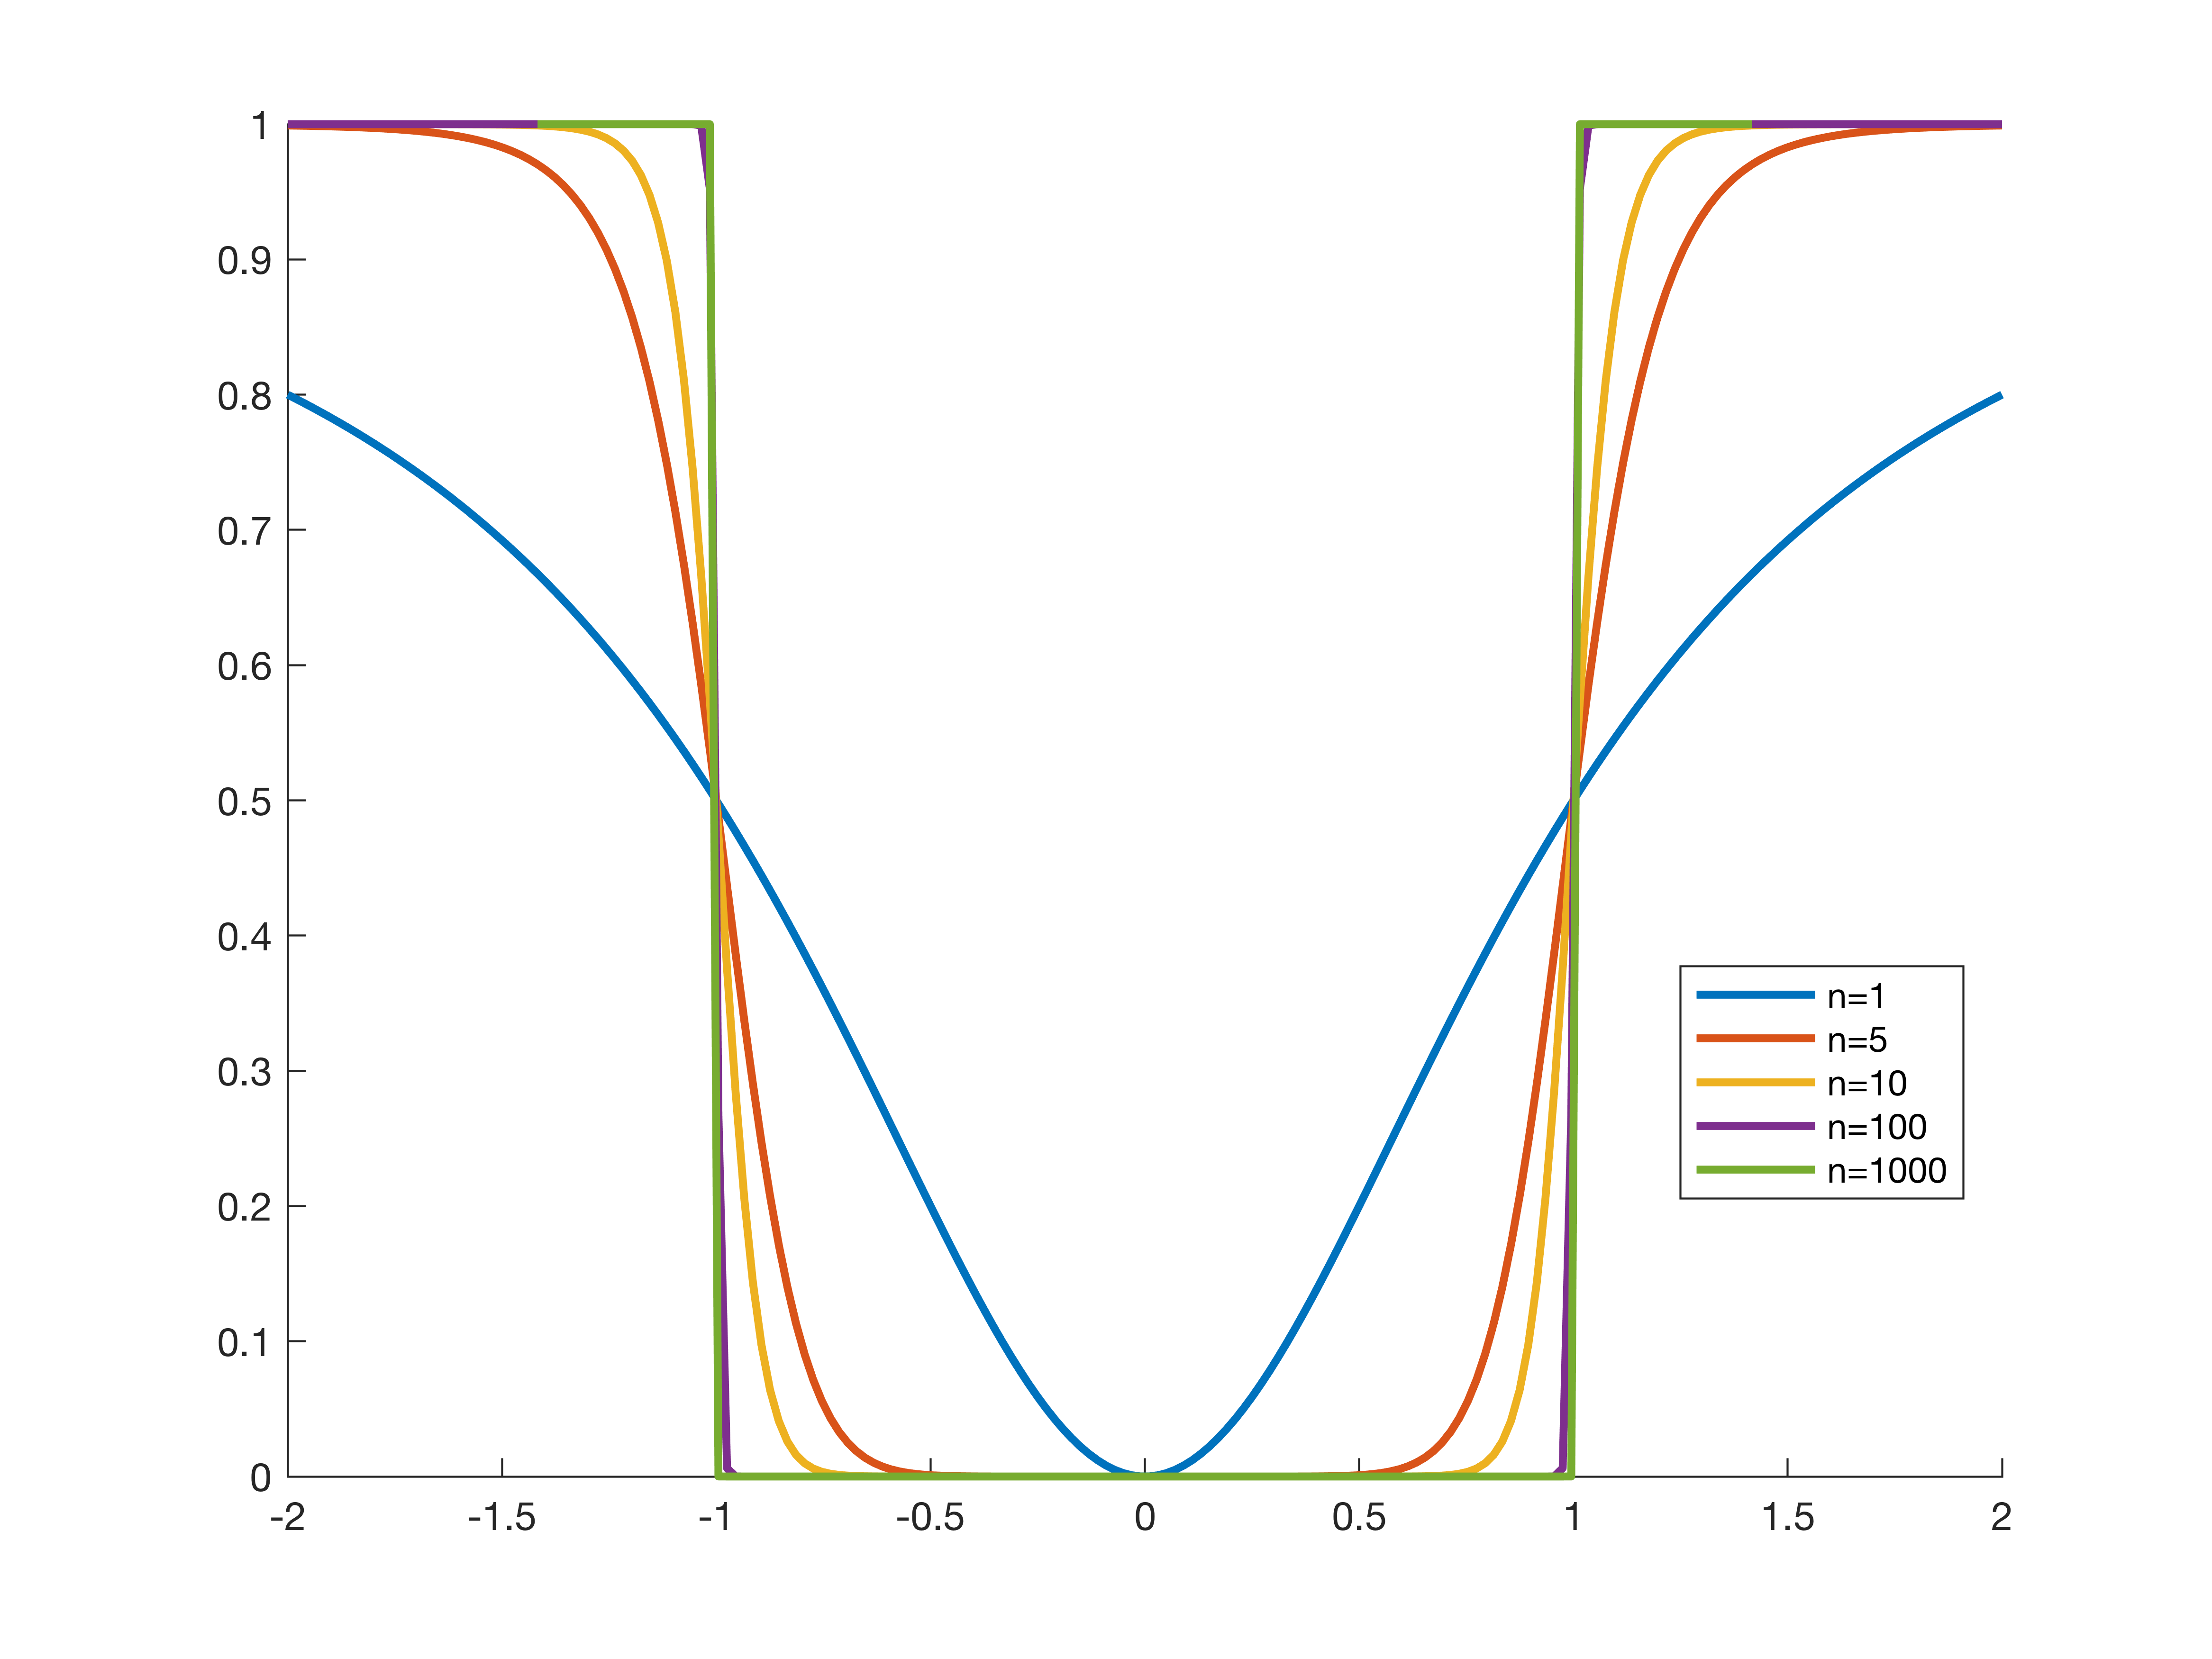
\includegraphics[width=.8\textwidth]{figure/fig1.png}
    %\includegraphics[width=2in]{XeTeX-2.jpg} 
    %\caption{An Numerical Example with $\alpha = 0.3, \beta = 0.98$}
%\end{figure}

\underline{Algorithm for finding $v^{*}$}

Consider following sequence $\{v_{n}\}_{n=0}^{\infty}$, where $v_{0}$ is some initial value $v_{0} \in [a, b]$:
\[
\begin{array}{ll}
    v_{1} &= T(v_{0})\\
    v_{2} &= T(v_{1}) = T(T(v_{0})) = T^{2}(v_{0})\\
    v_{3} &= T(v_{2}) = T(T^{2}(v_{0})) = T^{3}(v_{0})\\
          &\vdots \\
    v_{n} &= T(v_{n-1}) = T^{n}(v_{0})
\end{array}
\]

\begin{theorem}[Contraction Mapping (Banach Fixed Point Theorem)]
    If $(S, \rho)$ is a \underline{complete} metric space and $T:S \to S$ is a contraction with modulus $\beta$, then
    \begin{enumerate}
        \item [a)] $T$ has a \underline{unique fixed point} $v^{*}$ in $S$.
        \item [b)] $\{v_{n}(v_{0})\}_{n=1}^{\infty} \to v^{*} ~ \forall v_{0} \in S$. 
    \end{enumerate}
\end{theorem}
\begin{proof}
    \underline{First, we need to show that $\{v_{n}(v_{0})\}_{n=1}^{\infty}$ is Cauchy.}

    Let $v_{0} \in S$ be an arbitary initial point in $S$ and form the sequence $\{v_{n}(v_{0})\}_{n=1}^{\infty}$ by using the recursion on $T$:
    \[
    \begin{array}{ll}
        v_{1} &= T(v_{0})\\
        v_{2} &= T(v_{1}) = T^{2}(v_{0})\\
              &\vdots \\
        v_{n} &= T(v_{n-1}) = T^{n}(v_{0})\\
        v_{n+1} &= T(v_{n}) = T^{n+1}(v_{0})
    \end{array}
    \]
    Since $T$ is a contraction, 
    \[
    \rho(v_{2},v_{1}) = \rho(T(v_{1}),T(v_{0})) \leq \beta \rho(v_{1},v_{0})
    \]
    i.e., the distance between two successive terms of $\{v_{n}\}$ is bounded and decreasing in $n$.
    \[
    \rho(v_{n+1},v_{n}) = \rho(T(v_{n}),T(v_{n-1})) \leq \beta \rho(v_{n},v_{n-1}) \leq ... \leq \beta^{n} \rho(v_{1},v_{0}) , \quad n = 1,2,...
    \]
    To show that $\{ v_{n} \}$ is Cauchy, consider for any $m > n$:
    \[
    \begin{aligned}
        \rho(v_{m},v_{n}) 
        & \leq \rho(v_{m},v_{m-1}) + \rho(v_{m-1},v_{n})\\
        & \leq \rho(v_{m},v_{m-1}) + \rho(v_{m-1},v_{m-2}) + \rho(v_{m-2},v_{n})\\
        & \vdots\\
        & \leq \underbrace{\rho(v_{m},v_{m-1})}_{\leq} + \underbrace{\rho(v_{m-1},v_{m-2})}_{\leq} + ... + \underbrace{\rho(v_{n+2},v_{n+1})}_{\leq} + \underbrace{\rho(v_{n+1},v_{n})}_{\leq}\\
        & \leq \beta^{m-1} \rho(v_1,v_0) + \beta^{m-2} \rho(v_1,v_0) + ... + \beta^{n+1} \rho(v_1,v_0)+ \beta^{n} \rho(v_1,v_0)\\
        & = \beta^{n} \sum_{i = 0}^{m-n-1} \beta^{i} \rho(v_1,v_0)\\
        & < \beta^{n} \sum_{i = 0}^{\infty} \beta^{i} \rho(v_1,v_0)\\
        &= \frac{\beta^{n}}{1- \beta} \rho(v_1,v_0)\\
        \Longrightarrow \rho(v_{m},v_{n}) &< \frac{\beta^{n}}{1- \beta} \rho(v_1,v_0)
    \end{aligned}
    \]
    Hence
    \[
    \lim_{n \to \infty} \frac{\beta^{n}}{1- \beta} = 0
    \]
    For $\epsilon >0$, choose sufficiently large $n$ and $m (> n)$ such that $\rho(v_{m}, v_{n}) < \epsilon$ \imp $\{ v_{n}(v_{0}) \}_{n=1}^{\infty}$ is Cauchy.

    \underline{Next, show that $v_{n} \Longrightarrow v^{*} \in S$}

    Since $(S, \rho)$ is complete and since $\{v_{n}\}$ is Cauchy,
    \[
    \lim_{n \to \infty} v_{n} = v^{*} \in S
    \]

    \underline{Now show that $v^{*}$ is a fixed point.}

    Since $\lim_{n \to \infty} v_{n} = v^{*}$,
    \[
    T(v^{*}) = T(\lim_{n \to \infty} v_{n} ) = \lim_{n \to \infty} T(v_{n} ) = v^{*}
    \]
    (By \textbf{Theorem 8.4}, $T$ is (uniformly) continuous.)

    \imp $v^{*}$ is a fixed point of $T(v)$.

    \underline{Finally, show that $v^{*}$ is unique.}

    Suppose that $v^{*}$ and $v^{**}$ are two different fixed points, i.e. $T(v^{*}) = v^{*}$ and $T(v^{**}) = v^{**}$.

    Since $T$ is a contraction, $\exists \beta \in (0,1)$ s.t.
    \[
    0 < \alpha \equiv \rho(v^{*}, v^{**}) = \rho(T(v^{*},) T(v^{**})) \leq \beta \rho(v^{*}, v^{**}) = \beta \alpha
    \]
    \imp
    \[
    \alpha \leq \beta \alpha \quad \text{for}~ \alpha >0, ~ 0 < \beta <1
    \]
    \imp $\alpha = 0$ \imp $\rho(v^{*}, v^{**}) = 0$ \imp $v^{*} = v^{**}$
\end{proof}

\begin{theorem}[Blackwell's sufficient condition for a contraction]
    Let $X \subseteq \R$ and let $B(X)$ be a space of bounded functions. $f: B(X) \to \R$ with the sup norm. Let $T:B(X) \to B(X)$ be an operator satisfying two conditions
    \begin{enumerate}
        \item \underline{Monotonicity}

        $\forall f, g \in B(X)$ and $f(x) \leq g(x)$ for all $x$,
        \[
        T(f)(x) \leq T(g)(x) ~ \forall x \in X
        \]
        \item \underline{Discounting}

        $\exists \beta \in (0,1)$ s.t. \[
        T(f+ \alpha)(x) \leq T(f)(x) + \beta \alpha
        \]
        $\forall f \in B(X), ~\forall \alpha \in \R_{+}, ~\forall x \in X.$ 
    \end{enumerate}
    Then $T$ is a contraction mapping with modulus $\beta$.
\end{theorem}
\begin{proof}
    For any $f, g \in B(X)$, \[
    f = f +g - g = g + (f-g) \leq g + ||f-g||
    \]
    Then \[
    T(f)(x) \leq T(g + ||f-g||)(x) \leq T(g)(x) + \beta ||f-g||
    \]
    \imp $ T(f)(x) - T(g)(x) \leq \beta ||f-g|| $

    By symmetry, we also have
    \[
     T(g)(x) - T(f)(x) \leq \beta ||f-g||, \quad \text{for all } x
    \]
    \[
    \Longrightarrow ||T(f) - T(g)|| \leq \beta ||f-g|| 
    \]
    Hence $T$ is a contraction mapping.
\end{proof}

\underline{Pseudocontraction}

$T:X\to X$ in a metric space $(S, \rho)$ is called a \underline{pseudocontraction mapping} if $~\forall x, y \in X, ~ x\neq y,$ \[
d(T(x),T(y)) < d(x,y).
\]

\underline{Note}: Every contraction is a pseudocontraction.

\underline{Correspondence}
\begin{center}
    \texttt{[Insert a graph here]}
\end{center}

\begin{itemize}
    \item Relation: Not all points in $X$ are related to points in $Y$
    \item Function: Every point in $X$ is related to a \underline{single} point in $Y$.
    \item Correspondence:Every $x$ is related to some points (a set) in $Y$.
\end{itemize}
\begin{lemma}
    Pseudocontraction has at most one fixed point.
\end{lemma}

\begin{definition}
    A correspondence $\phi : X \rightrightarrows Y $ is a rule that assigns to every element $x \in X$ a non-empty subset $\phi(x) \subseteq Y$.
\end{definition}

\begin{center}
    \texttt{[Insert four graphs here]}
\end{center}



























%$$##
\clearpage
\section*{References}
%\beginrefs
%\bibentry{CW87}{\sc D.~Coppersmith} and {\sc S.~Winograd}, 
%``Matrix multiplication via arithmetic progressions,''
%{\it Proceedings of the 19th ACM Symposium on Theory of %Computing},
%1987, pp.~1--6.
%\endrefs

% **** THIS ENDS THE EXAMPLES. DON'T DELETE THE FOLLOWING LINE:

\end{document}




















